\hypertarget{TcpComBny_8cpp}{}\section{Référence du fichier src/\+Tcp\+Com\+Bny.cpp}
\label{TcpComBny_8cpp}\index{src/\+Tcp\+Com\+Bny.\+cpp@{src/\+Tcp\+Com\+Bny.\+cpp}}
{\ttfamily \#include $<$Tcp\+Com\+Bny.\+h$>$}\newline
{\ttfamily \#include $<$string$>$}\newline
{\ttfamily \#include $<$cstddef$>$}\newline
{\ttfamily \#include $<$cstdio$>$}\newline
{\ttfamily \#include $<$unistd.\+h$>$}\newline
{\ttfamily \#include $<$string.\+h$>$}\newline
{\ttfamily \#include $<$sys/types.\+h$>$}\newline
{\ttfamily \#include $<$sys/socket.\+h$>$}\newline
{\ttfamily \#include $<$netinet/in.\+h$>$}\newline
{\ttfamily \#include $<$arpa/inet.\+h$>$}\newline
Graphe des dépendances par inclusion de Tcp\+Com\+Bny.\+cpp\+:\nopagebreak
\begin{figure}[H]
\begin{center}
\leavevmode
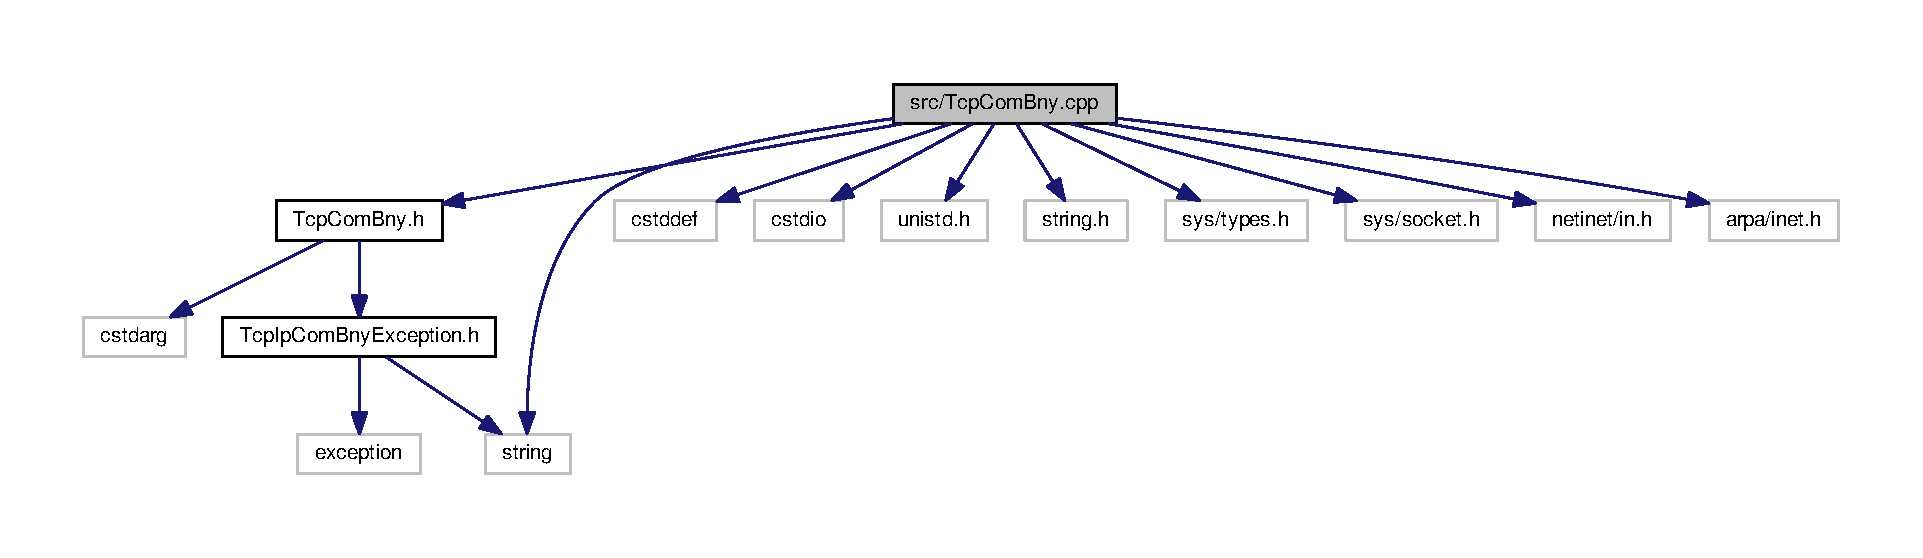
\includegraphics[width=350pt]{TcpComBny_8cpp__incl}
\end{center}
\end{figure}
